\subsection{Handling Cache Misses with \Sys Fallback}
\label{sec:cache_misses}

We now discuss how we optimize the handling of cache misses in \Sys, and propose an optimal strategy for picking the backup speculator based on the batch size.

\subsubsection{Algorithm}
We design \Sys's cache miss strategy based on the observation that cache misses occur \textit{almost certainly} at large batch sizes, and that when this happens, in SSD the \textit{whole batch} must wait for the backup speculator to complete before being verified.
We propose the \textit{\Sys fallback strategy}:
set the backup speculator to be equal to the primary speculator at low batch size, then switch to a low-latency speculator ~\citep{suffixtree,infinigram,infini_mini} for larger batch sizes $b>b^*$, where the critical batch size $b^*$ is derived in the following section. 


\subsubsection{Theoretical Results}
We prove that \Sys's backup speculator strategy is optimal, under the conditions that SSD uses a high-quality (slow) speculator (primary), and a lower-quality (fast) speculator (backup). We begin with a corollary to Theorem~\ref{thm:speedup} which accounts for the impact of batch size on the expected speedup attained by SSD.
This result assumes that in SSD the whole batch waits for the backup speculator to complete before verifying the batch.

\begin{corollary}
\label{cor:speedup_with_batch_size}
At batch size $b$, the expected speedup from SSD is equal to:
\begin{eqnarray*}
speedup &=& \frac{p_{\mathrm{hit}} \cdot E_{\mathrm{hit}} + (1-p_{\mathrm{hit}}) \cdot E_{\mathrm{miss}}}{p_{\mathrm{hit}}^b \cdot \max(1, T_p) + (1-p_{\mathrm{hit}}^b) \cdot (1 + T_b)}, \quad \text{which approaches} \\
% \end{eqnarray*}
% As $b \rightarrow \infty$, this approaches:
% \begin{eqnarray*}
    && \frac{p_{\mathrm{hit}} \cdot E_{\mathrm{hit}} + (1-p_{\mathrm{hit}}) \cdot E_{\mathrm{miss}}}{1 + T_b} \quad \text{as } b \rightarrow \infty.
\end{eqnarray*}
\end{corollary}
% \color{red}
In our implementation, the backup strategy is to return random tokens,\footnote{Note that we can easily improve upon this random token strategy by using extremely fast non-neural speculators, like those based on n-grams~\citep{infinigram,suffixtree}.} and the primary strategy is to do just-in-time speculation. 
As the batch size increases, the entire batch stalls on the latency of the backup speculator as cache misses happen more frequently.
This forces the choice of a low latency speculator at larger batch sizes, as the following theorem makes precise. 
\color{black}

\begin{theorem}
\label{thm:cache_miss}
The optimal fallback strategy for cache misses, given two speculators of varying speeds and quality, is to use the slow and accurate speculator as the backup for batch sizes $b < b^*$, and the fast speculator otherwise.
We solve for $b^*$ in Appendix \ref{app:theory}. 
\end{theorem}


\subsubsection{Empirical Evaluation}
We show in Figure~\ref{fig:bsz} (left) that as the batch size increases, using a fast backup speculator that returns random tokens outperforms using a slow but more accurate neural speculator just-in-time.
We note that for all of these batch sizes, we use fan-out $F=1$ and 1 H100 GPU for drafting.
In Figure~\ref{fig:bsz} (right) we show that we can reduce latency further by scaling draft-time compute.
Specifically, we show the projected speedups we would get at batch size 16---computed based on our cache hit rate curves (Figure~\ref{fig:geom})---if we increase the number of draft GPUs (and thus, the fan-out factor).
% We also see that we can reduce latency by scaling draft-time compute.
Dedicating more devices to speculation leads to larger speculation caches and thus higher cache hit rates. 

\begin{figure}[H]
    \centering
    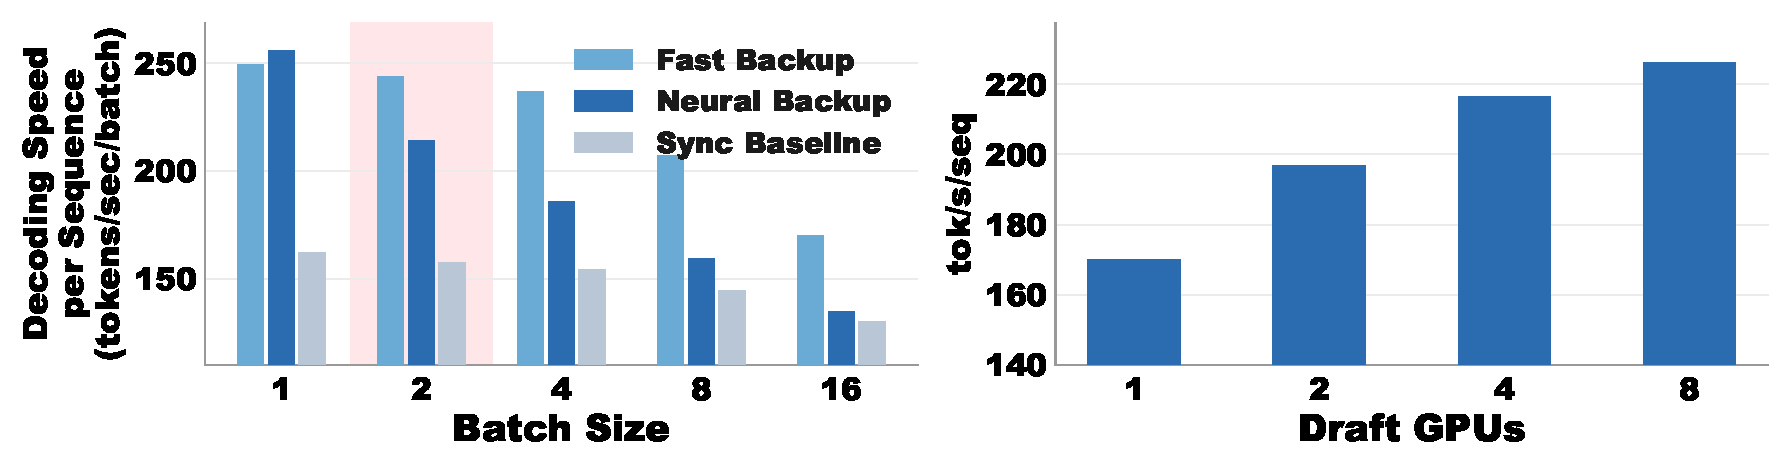
\includegraphics[width=\linewidth]{figures/batch_scaling.pdf}
    \caption{(Left) Optimal backup speculator (fast vs neural) depends on batch size, as Theorem \ref{thm:cache_miss} predicts (temperature 0). 
    (Right) We forecast how decoding speed improves with draft compute (and thus, fan-out) for batch size 16 with the fast backup speculator.
    At large batch sizes we become compute bound, speedups more GPUs to drafting.
    }
    % (Right) We forecast how cache hit rate/decoding speed improves with draft compute (fan out) at temperature 1.0 when cache hit rate is 0.6 with one draft device. }
    \label{fig:bsz}
\end{figure}